\chapter{Literature Review}
\label{cha:literature-review}

This research covers multiple fields of study, therefore an extensive
literature review covering these fields is necessary. This section starts with a
look at the field of \emph{narratology}, or narrative theory, to gain some
insights into the themes and components that make up stories. Looking at
different formalisms that have been created for narrative and which themes and
motifs recur in stories should better inform the creation of techniques with
which to generate stories.

We also examine current approaches to interactive narrative generation,
focussing particularly on the use of planners, drama managers, social norms and
logical modelling for describing stories. Most of these implementations are
designed with multi-agent systems in mind, where the story forms a set of rules
which govern these agents. The start of this part of the literature survey also
examines non-interactive story generation through means of techniques such as
generative grammar, in order to provide a historical context for the research
that follows. 

As part of the examination of implementations of interactive narrative, this review especially focuses on agent-based systems. The section concludes with an overview of emotional models that can be used to model distinct characters using agents.

\section{Narratology}
\label{sec:narratology}
Narratology is a deep field with many sub-fields. This review examines the parts of it that might best inform the modelling of narrative by computers, as well as the construction of interactive narrative.

The first part of the overview of narratology examines research into categorising different types of narrative, both traditional and experimental.
This draws from classic narratological texts, as well as work done on
``cybertext'' and experimental narrative in the interactive age. This
examination of recent research into non-linear narratives is essential for the
construction of interactive narratives for games or simulations.

Structuralist formalisms of narrative attempt to explain how stories work by dividing them into commonly occuring themes and motifs. This is a natural fit to the modelling of narratives by computer, especially if using an ontology. This overview of narratology starts with structuralism for this reason.

After the overview of structuralists' narrative models follows a section on the use of formal logic for narrative modelling. The section ends with descriptions of other types of story components, taxonomies and ontologies used in the literature.

\subsection{Narrative Structure}
What is the difference between a narrative and a sequence of events? If we
recount the events that happened to us during the course of a day, would that
``count'' as a narrative? When is the retelling of events a simple listing of
facts, and when is it a story?

Narratologists from \citep{bal2009narratology} onwards refer to the
chronological ordering of events as \emph{fabula} (from the Russian фабула, ``scene''), and the retelling and
reordering of those events in a narrative as \emph{syuzhet} (сюжет, ``plot'').
In fact, Russian structuralists Propp~\cite{propp1968morphology} and
Shklovsky~\cite{shklovsky1991theory} were the first to use these terms in the
context of narrative, before their rediscovering by modern narrative theorists.

The concepts of \emph{fabula} and \emph{syuzhet} are key to the understanding of
narrative structure. Thanks to Aristotle's
\emph{Poetics}~\cite{halliwell1968aristotle}, we understand that a story must
have a beginning, a middle and and end. These three parts of a story describe
how the \emph{syuzhet} are organised, which can refer to its \emph{fabula}
(chronological) events in any order. For example, the beginning of a movie could
be set at the present day in the life of the protagonist, the middle could be a
flashback to an earlier time in her life, and the end could return to the events
following the start of the movie.

Though Aristotle identifies the beginning, middle and end as three key story
divisions, other theorists divide the \emph{syuzhet} of a story further. Joseph
Campbell's work \emph{The Hero with a Thousand Faces}~\cite{campbell2008hero}
describes how almost every story is a variation of the \emph{Hero's Journey}
(also called the \emph{monomyth}). Like Aristotle's beginning, middle and end,
the Hero's Journey has three acts: the Departure, the Initiation and the Return.
Campbell divides these acts further into seventeen distinct stages:

\paragraph{Departure}
\begin{enumerate}
  \item The Call to Adventure
  \item Refusal of the Call
  \item Supernatural Aid
  \item Crossing the Threshold
  \item Belly of the Whale
\end{enumerate}
\paragraph{Initiation}
\begin{enumerate}[resume]
  \item The Road of Trials
  \item The Meeting with the Goddess
  \item Woman as Temptress
  \item Atonement with the Father
  \item Apotheosis
  \item The Ultimate Boon
\end{enumerate}
\paragraph{Return}
\begin{enumerate}[resume]
  \item Refusal of the Return
  \item The Magic Flight
  \item Rescue from Without
  \item The Crossing of the Return Threshold
  \item Master of Two Worlds
  \item Freedom to Live
\end{enumerate}

In summary, the hero begins the story at home or in some otherwise familiar
setting, where she is called away on an adventure. After possibly rejecting this
call, the hero leaves home (crosses the threshold) and sets off for the land of adventure. After facing
many trials and possibly defeating an enemy, the hero returns home once again.
Having endured the many trials of the journey, our hero becomes stronger in spirit
and character.

As a classic example, consider the plot of Tolkien's \emph{The Hobbit}. At the
start of the tale, Bilbo Baggins is a comfortable but risk-averse hobbit who
refuses to leave his comfortable surroundings when Gandalf first visits him to
send him on a quest. Of course, he does eventually leave home to fulfill the
quest, returning home a changed character.

Campbell argues that the \emph{monomyth} acts as a shared cultural memory of
sorts, being the universal template for the rite-of-passage tale. He says that
it is passed down as myth through many different cultures, replicating in much the same way
as genes (or memes) do and that it can be thought of as a \emph{metamyth}, or the
spiritual history of humanity.

\subsection{Types of Narrative}
% Author Kurt Vonnegut
% Look at Cybertext, etc, and try to explain how best to divide different types
% of story
The rise of the Web in the 1990s brought with it great interest in the future of narrative in cyberspace. Aarseth's work, \emph{Cybertext} \citep{aarseth1997cybertext} describes the creation of a new form of narrative, for which he coins the term \emph{ergodic literature} (from the Greek words \emph{ergon} and \emph{hodos}, meaning `work' and `path'). In this new form of narrative, some amount of work or effort is required by the reader in order to traverse the path that the story takes.

% scriptons/discourse textons/fabula (Bal 1997)
Aarseth makes a distinction between the narrative as written by the author, and the way in which it is traversed by the reader, calling the former \emph{textons} and the latter \emph{scriptons}. In ergodic literature, the \emph{scripton} is produced by the effort that the reader goes through in interpreting the \emph{texton}. In the context of a game, it is as though the game interface is a gateway that allows access to the narrative at different times. Using classical music as a metaphor, the texton can be thought of as the \emph{score}, and the scripton the \emph{performance}.

% TODO Make sure you update the intro with this
In section \ref{sec:generative-and-interactive-narrative}, we assert that how generative a narrative is and its level of interactivity are two different variables in an experimental narrative. However, Aarseth identifies seven different methods of story traversal: \emph{dynamics, determinability, transiency, perspective, access, linking and user function}.

\paragraph{Dynamics} describe whether or not the content and number of scriptons changes. In a simple, static story with branching choices (such as in a \emph{Choose your own adventure} story), both the number of textons and scriptons are fixed, since all paths have been written out beforehand. A dynamic story would still have a fixed number of textons, but the scriptons would be generated as the user traverses the path of the narrative.
\paragraph{Determinability} is how deterministic the narrative is, whether or not the same interactions will result in the same scripton being produced.
\paragraph{Transiency} means to what extent scriptons are produced as time flows, or whether user interactions are required to produce them.
\paragraph{Perspective} is whether or not the user/reader plays a role as a character in the narrative.
\paragraph{Access:} if a user has access to all scriptons at any point in traversing the narrative, or whether their access is restricted.
\paragraph{Linking} means whether or not parts of the scripton are linked to other parts, and whether these links are conditional (if they rely on a user having already traversed part of the scripton).
\paragraph{User functions:} the functions the user uses to traverse the text. This could be interpretive (which is implicit in any traversal of the text), explorative (traversing the scripton according to whim) or configurative (specifying parts of the scripton in advance), for example.

% Ugh, this is all so arbitrary. Go on to describe Aarseth's PCA of these variables and explain why you don't think it's a good fit.

By performing correspondence analysis (a process similar to principle component analysis) on a diverse corpus of 23 texts ``\emph{ranging from ancient China to the Internet}'', Aarseth filters these seven variables down into two numerical axes which account for 49 percent of the variation between stories. Using these axes, he groups classic tales such as \emph{Moby Dick} and more experimental narratives such as William Gibson's \emph{Agrippa} and Michael Joyce's \emph{Afternoon}. By grouping these stories into categories, he intends to show how emerging media are enabling new types of story.

Chris Crawford's \emph{Chris Crawford on Interactive Storytelling} \citep{crawford2012chris} provides a scathing assessment of the relationship between narrative theory and computer science. A veteran of the games industry, he argues that `soft' science theories such as those of Aarseth et al are entirely removed from `hard' science, and are therefore an example of bubble intellectualism and impossible to implement. 

Crawford himself provides a useful examination of experimental narrative in computer games, defining interactivity as:

\begin{quote}
A cyclic process between two or more active agents in which each agent alternately listens, thinks, and speaks.
\end{quote}

He argues that for game narratives to be truly interactive, they must be more social. Characters in a story must be able to react with the player as though they were people in real life. In turn, the player should have some degree of freedom in the way in which they interact. Rather than presenting branching story points as choices, a better way to interact would be socially, through talking to agents in the game. This is the approach that Fa\c{c}ade takes \citep{mateas2003faccade}, which Crawford acknowledges as the most successful attempt at interactive storytelling to date. A detailed description of Fa\c{c}ade's implementation appears in section \ref{sec:modelling-agents}.

In order to determine whether Crawford's assertion that narratology research is
too far removed from its practical implementations to be of use, provide an
overview of these implementations and their underlying research in section \ref{sec:implementations}. Has narrative theory research informed the creation of computer-generated or interactive narrative at all, or do they all take approaches grounded in computer science and artificial intelligence? If narrative theory has not been used, then we must ask another question: why not?


\subsection{Structuralist Formalisms of Narrative}
% Propp, etc
Attempts to organise recurring themes, roles and motifs of narrative go back at least a century. The Aarne-Thompson tale-type index \citep{aarne1987types}, first published in 1910 and later refined by Stith Thompson in 1928 and 1961, is well known amongst folklorists as a classification and analysis method for traditional folktales and myths. Aarne-Thompson's index is a taxonomy of tale themes, arranging tales into categories such as \emph{animal tales} and \emph{jokes and anecdotes}, and then sub-categories (\emph{tales of magic} and \emph{numskull [sic] stories} being two examples). This taxonomy is only two levels deep however, and only serves as a useful way to categorise individual stories or tales. In order to break down and analyse components of tales, we must dig deeper.

In \emph{Structural Anthropology}, Claude L\'{e}vi-Strauss seeks to discover why myths and legends are so similar across cultures and history \citep{levi2008structural}. He concludes that there are global laws that govern the way in which people create stories, therefore these laws can be modelled as a set of rules for describing myths.

His theory is that myths describe opposing forces which are resolved through mediation. The example he gives in \emph{Structural Anthropology} describes how Native American legends often contain `trickster' characters in the form of ravens or coyotes. As scavenging animals, these tricksters symbolically act as mediators between life and death.

Like much of early narrative theory, there is no rigorous evaluation of L\'{e}vi-Strauss' ideas, leaving them feeling a little too opinionated and arbitrary. While interesting, L\'{e}vi-Strauss' ideas bring us no closer to developing a formal model of narrative structure. For that, we must go even further back in time, and turn to Vladimir Propp.

\subsubsection{Propp's Morphology of the Folktale}
A notable narrative structuralist is Vladimir Propp, creator of \emph{The Morphology of the Folktale}~\cite{propp1968morphology}, a formalism for Russian folktales. Propp's formalism, though originally limited in scope, generalises well, and is still used by researchers to procedurally generate stories~\cite{grasbon2001morphological,gervas2005story,hartmann2005motif}. Drawing from a corpus of one hundred Russian folktales, Propp identifies thirty-one distinct \emph{story functions}, each of which is identified with a number and symbol. These functions are executed by characters following certain roles, each of which has a \emph{sphere of action} consisting of the functions that they are able to perform at any given point of the story. Stories are created by chaining story functions together, with subplots expressed as parallel chains of story functions.

In this formalism, characters have \emph{roles}, such as \emph{hero}, \emph{villain}, \emph{dispatcher}, \emph{false hero}, and more. Characters performing a certain role are able to perform a subset of \emph{story functions}, which are actions that make the narrative progress. For example, the \emph{dispatcher} might send the \emph{hero} on a quest, or the \emph{victim} may issue an \emph{interdiction} to the \emph{villain}, which is then \emph{violated}.

Propp defines a total of 31 distinct story functions, each of which is given a number and symbol in order to create a succinct way of describing entire stories. Examples of such functions are:

\begin{itemize}
  \item One of the members of a family absents himself from home: \emph{absentation}.
  \item An interdiction is addressed to the hero: \emph{interdiction}.
  \item The victim submits to deception and thereby unwittingly helps his enemy: \emph{complicity}.
  \item The villain causes harm or injury to a member of the family: \emph{villainy}.
\end{itemize}

Each of these functions can vary to some degree. For example, the \emph{villainy} function can be realised as one of 19 distinct forms of villainous deed, including \emph{the villain abducts a person}, \emph{the villain seizes the daylight}, and \emph{the villain makes a threat of cannibalism}.

These functions are enacted by characters following certain roles. Each role (or \emph{dramatis personae} in Propp's definition) has a \emph{sphere of action} consisting of the functions that they are able to perform at any point in the story. Propp defines seven roles that have distict spheres of action: \emph{villain}, \emph{donor}, \emph{helper}, \emph{princess}, \emph{dispatcher}, \emph{hero}, and \emph{false hero}.

Though Propp defines each \emph{dramatis personae} as being distinct (characters can only play one role at a time), it is simple to extend the idea to allow for overlapping roles. For example, a victim could also be a donor, so the set of functions they can perform would be the union of both the victim and donors' permitted function sets. Propp does not explore this possibility in \emph{The Morphology of the Folktale}, however.

\begin{figure}[!t]
\centerline{
\includegraphics[height=0.4in]{propp1.png}}
\caption{One Propp function following another}\label{fig:propp1}
\end{figure}

\begin{figure}[!t]
\centerline{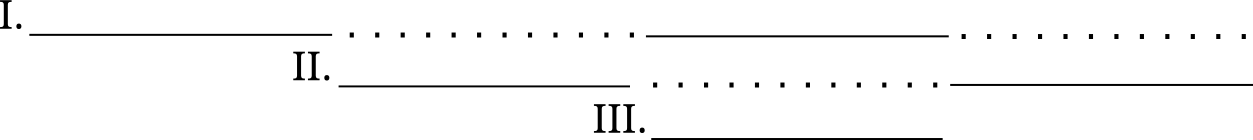
\includegraphics[height=0.6in]{propp2.png}}
\caption{Multiple simultaneous functions}\label{fig:propp2}
\end{figure}

In a typical story, one story function will follow another as the tale progresses in a sequential series of cause and effect (figure~\ref{fig:propp1}). However, Propp's formalism also allows for simultaneous story functions to be occuring at once (figure~\ref{fig:propp2}).

Though flexible, Propp's formalism is limited in its expressiveness. All story functions describe events at the same level of abstraction, describing one event after another. Also, Propp insists that the story functions occur in a prescribed order. Later French structuralists such as \citep{bremond1980logic}, \citep{greimas1983structural} and~\citep{todorov1969grammaire} address the latter problem by generalising Propp's work outside of Russian Folktales, though each represents only incremental improvements on Propp, lacking a means of nesting story functions to create abstractions. \citep{barthes1975introduction} broadly describe hierarchically composing \emph{narrative units} but, lacking implementation details, these can only be used as a template from which to build a new narrative model.
% What are the shortcomings of Propp? (i.e. lack of abstractability, etc)

% \subsection{Describing Stories with Logic}
% Laure-Ryan did a bit of this, also include linear logic approaches

\subsection{Other Types of ``Story Component''}
Lehnert's \emph{plot units} are a more recent narrative formalism \cite{lehnert1981plot}. However, these plot units only describe stories as three types of event: positive, negative and mental. These events occur with respect to a single character in the story, so an author must always author story components with concrete characters in mind, making them difficult to re-use. Similarly to Propp's system, the order of composition must always be in a certain sequence, and plot units cannot refer to other plot units. Again, we are left without a means of creating abstractions for our story components. In the ``TropICAL: a DSL for Tropes'' section, we describe how tropes allow the nesting of components to allow story authors to create their own abstractions, addressing this issue.

\section{Implementations of Experimental Narrative}
\label{sec:implementations}
% I've plenty of material, but it really needs reworking and extending

\subsection{Story Generation}
% TaleSpin, etc
Inspired by Chomsky's theories of generative grammar \citep{chomsky1968sound}, researchers in generative narrative strive to build their own `universal grammar' for narrative.

\begin{figure}[!t]
  \begin{center}
  \begin{enumerate}
    \item $\texttt{Attempt}\rightarrow \texttt{Plan} + \texttt{Application}$\\
           $\qquad\Rightarrow\texttt{MOTIVATE(Plan, Application)}$
    \item $\texttt{Application}\rightarrow\texttt{(Preaction)*} + \texttt{Action} + \texttt{Consequence}$\\
           $\qquad\Rightarrow\texttt{Allow(AND(Preaction,Preaction,...),}$\\
           $\qquad\{\texttt{CAUSE | INITIATE | ALLOW}\}\texttt{(Action,Consequence)}$
  \end{enumerate}
  \end{center}

  \caption{Example rules from Rumelhart's story grammar}\label{fig:rumelhart}
\end{figure}

\citet{rumelhart1975notes} is one early and influential model for the grammatical generation of natural language. Figure \ref{fig:rumelhart} shows two example rewrite rules from this grammar. The `+' symbol denotes items happening in a sequence, the `\textbar' showing possible alternatives. `*' denotes one or more item being generated. Capitalised words (such as ALLOW, MOTIVATE, etc) describe relationships between items. For example, MOTIVATE is a relationship between a character's thought and their reaction to that thought.

This generative grammar approach can be seen in systems such as Pemberton's GESTER \citep{pemberton1989modular}, which generates stories based on a grammar synthesised from old French epic tales. \citet{lang1999declarative} describe a declarative model for narrative, consisting of lists of first-order predicate calculus expressions. These expressions describe events, states, goals and beliefs which combine to form a narrative. More specifically, it combines:

\begin{itemize}
  \item A \textbf{grammar interpreter} to search for a sequence of grammer rewrites which would produce a convincing narrative.
  \item A set of \textbf{temporal predicates} to describe the occurence of events over time and enforce temporal constraints on story components.
  \item A \textbf{world model} which describes the set of actions that characters may perform and fluents that may alter over the course of the narrative.
  \item A \textbf{natural language output unit}, which takes the sequence of events produced by the story grammar and converts it into readable natural language sentences.
\end{itemize}

This combination of using a grammar interpreter, world model and natural language output unit is especially common amongst generative grammar approaches.

While generative grammar approaches may be effective for procedurally creating prose, they are less well suited to the creation of \emph{interactive} narratives. Once the grammar rewrite rules are specified, the user is entirely passive, unable to affect the way in which the story is bein generated. For this to happen, the narrative needs to be part of a system that reacts to the actions of the user, such as a computer game.

\begin{figure}[!t]
\begin{quote}
  ONCE UPON A TIME GEORGE ANT LIVED NEAR A PATCH OF GROUND. THERE WAS A NEST IN AN ASH TREE. WILMA BIRD LIVED IN THE NEST. THERE WAS SOME WATER IN A RIVER. WILMA KNEW THAT THE WATER WAS IN THE RIVER. GEORGE KNEW THAT THE WATER WAS IN THE RIVER. ONE DAY WILMA WAS VERY THIRSTY. WILMA WANTED TO GET NEAR SOME WATER. WILMA FLEW FROM HER NEST ACROSS THE MEADOW THROUGH A VALLEY TO THE RIVER. WILMA DRANK THE WATER. WILMA WASN'T THIRSTY ANYMORE.

GEORGE WAS VERY THIRSTY. GEORGE WANTED TO GET NEAR SOME WATER. GEORGE WALKED FROM HIS PATCH OF GROUND ACROSS THE MEADOW THROUGH THE VALLEY TO A RIVER. GEORGE FELL INTO THE WATER. GEORGE WANTED TO GET NEAR THE VALLEY. GEORGE COULDN'T GET NEAR THE VALLEY. GEORGE WANTED TO GET NEAR THE MEADOW. GEORGE COULDN'T GET NEAR THE MEADOW. WILMA WANTED TO GET NEAR GEORGE. WILMA GRABBED GEORGE WITH HER CLAW. WILMA TOOK GEORGE FROM THE RIVER THROUGH THE VALLEY TO THE MEADOW. GEORGE WAS DEVOTED TO WILMA. GEORGE OWED EVERYTHING TO WILMA. WILMA LET GO OF GEORGE. GEORGE FELL TO THE MEADOW. THE END.
\end{quote}
\caption{Example TALE-SPIN output}\label{fig:tspin}
\end{figure}

% TODO elaborate on this
Lebowitz' UNIVERSE system \citep{lebowitz1985story} focuses on the creation of believable characters, using `plot fragments', or short plans, to generate story outlines for soap operas.

James Meehan's TALE-SPIN \citep{meehan1977tale} is an influential early approach to story generation using planning. In TALE-SPIN, the author describes a story domain, its characters and their goals, and a natural language story is produced as output. It works by using a problem-solver to resolve each character's goals over the story domain. Figure \ref{fig:tspin} is an example of TALE-SPIN's output.

TALE-SPIN's strong planning component is evident in the reading of its output. Sentences are terse, with one event leading directly to another in order to achieve some goal. One problem with this character-led approach is that the goals of the author are not necessarily taken into account. If the author intends for a character to die at some point in the story, it seems unnatural for a character to have the goal of dying to fulfill this intention.

 Turner criticises TALE-SPIN's stories as seeming ``pointless and somewhat boring'' \citep{turner1986thematic}, going on to create the MINSTREL system for story generation \citep{turner1993minstrel}. Using the legendary world of King Arthur's court as a story domain, MINSTREL strives to generate stories with an authorial purpose.

MINSTREL attempts to address TALE-SPIN's shortcomings by introducing two types of schema: author-schemas and character-schemas, both of which combine to represent the elements of a story. The author-schemas describe the goals of the author of the system, allowing story creators more control over the structure and content of their narrative. This allows authors to specify a `point' or moral to their story, something that is not possible to achieve with TALE-SPIN. Character-schemas describe character-level goals in a similar manner to those of TALE-SPIN's.

The comparison of TALE-SPIN and MINSTREL highlights a challenge that has dominated story generation for decades: the balance of \emph{character} and \emph{plot}. Especially with approaches based on multi-agent systems, the regulation of character actions to conform to an underlying theme or structure is a challenging problem.

However, modelling characters with agents is a promising approach to take in order to gain a story which is both generative and interactive. In such a system, an author can specify the story world and character models, creating the `big picture', and the agents would be able to fill in the details (such as dialogue, sub-plots, and relationships).

An apt metaphor would be that of animation. In large animation studios such as Disney, the lead animator draws the key frames of a sequence, and a team of other animators works to fill in the gaps in between. This is what the combination of a managed narrative with agents could achieve: the author would be the `lead animator' in such a system, with the agents being the assistants.

So far into this literature review, we have some idea of where a promising approach may lie. However, the implementations until now have still focused mainly on \emph{generation\/}, and little on \emph{interaction\/}. Character models have been mentioned, but these do not react in real time to a user. For that, we need a multi-agent system.

\subsection{Intelligent Agents as Characters}
% Write an introduction
Story worlds are usually populated with characters. Interactive story worlds
such as games contain characters with very basic scripted behaviour. At even the
highest level of game character simulation, AI techniques are usually used to
govern basic behaviour such as movements and actions. Governing character
behaviour to fit within the context of a narrative is a more challenging
problem. This section examines different approaches to tackling this challenge.

\subsubsection{Planner-based Systems}
The most prevalent approach to the generation and management of plot in
interactive narrative is to use planners. With a planner, an author sets the
goals for the story (certain situations that they would like to see happen), and
the planner tells the character agents what to do to make sure these ``story
goals'' are achieved. When a player that is interacting with the system takes an
action that compromises the story goals, the planner must re-plan to make sure
the goals can still be achieved, by restricting the actions of the player or
intervening in some other manner.

% This needs elaboration
\citep{young1999notes} argues that planners are a good method for regulating
plot, later creating the \emph{Mimesis} architecture for integrating a planner with character agents in an interactive game environment \cite{young2004architecture}. Young describes how narrative systems must re-plan when a player makes  narrative-breaking actions, by either restructuring the narrative mid-story (\emph{accommodating} the action) or preventing the action from executing (\emph{intervening} on the action).

Given its influence over subsequent approaches to interactive narrative
generation, it is worth looking at the Mimesis architecture more closely.
It is designed to integrate into the \emph{Unreal
  Tournament} game engine, and has five components: the \emph{mimesis
  controller}, the \emph{story planner}, the \emph{discourse planner}, the
\emph{execution manager} and the \emph{MWorld}.

Figure \ref{fig:mimesis} shows how this components work together to form the
Mimesis architecture. Once an author has created the pre-defined libraries of
actions needed by the story planner, the following steps are taken to determine
the course of the story:

\begin{enumerate}
  \item All the components connect to the Mimesis Controller (MC) via socket
    connection. It then acts as a message router.
  \item The game initiates a plan request containing the state of the game
    world, a list of possible actions, and the goals for the plan.
  \item The \emph{story planner} responds with a \emph{story world plan}, a data
    structure that describes the actions (selected from the list) that must occur over time in order to
    meet the plan request's goals.
  \item Once the story world plan is created, it is sent to the \emph{discourse
      planner}, along with a list of actions that can occur in the game engine
    (such as camera movements, voice-overs and background
    music). The discourse planner then creates a sequence of these actions that
    best fit the story world plan.
  \item The discourse planner then sends the narrative plan to the
    \emph{execution manager}, which builds a directed acyclic graph (DAG), where
    the nodes are the actions within the plan and the edges are the temporal
    constraints between the orderings of the actions. The execution manager
    removes nodes from the DAG in order, sends the node's actions to the
    game engine, and updates the graph.
  \item The \emph{MWorld} is essentially the environment in which the story
    occurs, consisting of the game engine, coordination code, and class
    definitions for actions, and discourse planners. It is the MWorld that
    receives actions from the execution manager to be executed, and executes
    these actions in the game engine.
\end{enumerate}

Mimesis uses DPOCL (Decomposed Partial-Order Causal-Link Planner)~\cite{young1994decomposition} plans for
its story planning. DPOCL plans are composed of \emph{steps} (the plan's
actions), \emph{ordering constraints}, \emph{decomposition links} describing the
hierarchical structure of a plan, and \emph{causal links} between pairs of
steps. It uses \emph{refinement search} \cite{kambhampati1995planning} as its
plan reasoning process, searching through the space of possible plans represented as a directed
graph, with each node in the graph being a plan or partial plan. Mimesis
specifies the initial planning problem for DPOCL using the current and goal
states of the story.

A key feature of Mimesis is its handling of user actions which potentially
interfere with the story plan, making its goals unachievable. Its two strategies
for mediating in such situations are \emph{intervention} and
\emph{accommodation}. In the intervention strategy, Mimesis simply prevents the
user's action from having any effect in the game world. With accommodation,
Mimesis replans the story events, restructuring the plan so that the interfering
actions are taken into account and worked around.

\begin{figure}[!t]
\centerline{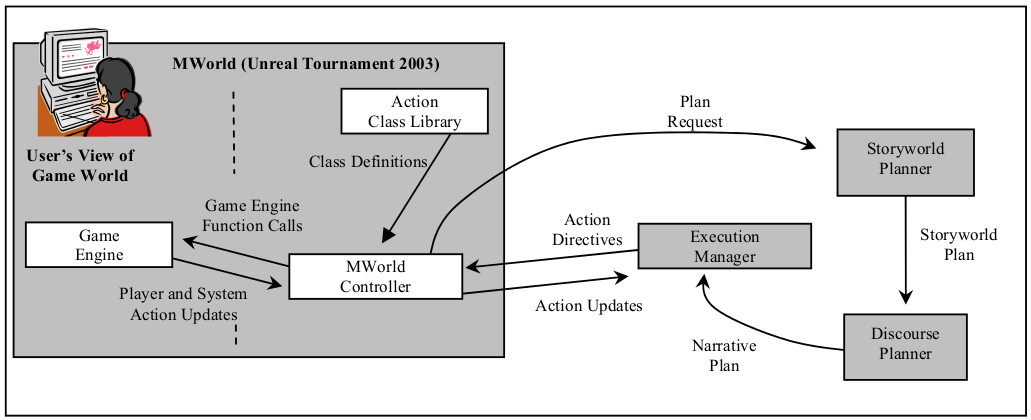
\includegraphics[height=0.4in]{mimesis.png}}
\caption{The Mimesis architecture, from \cite{young2004architecture}}\label{fig:mimesis}
\end{figure}

% This needs elaboration
Cavazza et al's \emph{I-Storytelling} system~\cite{cavazza2002character} implements Young's architecture with ideas from Barthes' narrative units, using characters with Hierarchical Task Networks (HTNs) to generate its stories. Each character has a main task, which is divided into subtasks to create a task hierarchy, with each task node having pre- and postconditions. The story emerges from the outcomes of each character's plans, and the narrative structure as a whole is not planned.

% This needs elaboration
\citep{riedl2003managing} describes further development of Young's architecture,
allowing the story author to create plans for the overall narrative in addition
to its characters, in order to have more control over narrative structure.
Rather than using a narrative model, this version of Mimesis models the player to track their expected level of suspense while interacting with the story. Like the \emph{I-storytelling} system, its plans are hierarchical, using the Longbow hierarchical partial-order causal link planning system~\cite{young1994decomposition}.

A disadvantage of these planner-based systems is that they require the story author to think in a planner-oriented manner. They must consider the goals of both the story and the character, plans to achieve these goals, and re-planning when goals are not met or when situations change. This is a drastic change from the usual story writing methods of authors, where the focus is on structure, plot, themes and characters. Though graphical user interfaces such as Mimesis' Bowman system~\cite{thomas2006author} could be used to assist planner-driven story authoring, a complete shift in creative workflow is still required, making them inaccessible to non-technical writers.

% This needs elaboration
\subsubsection{Drama manager-based Systems}

Carnegie Mellon University's OZ project \cite{mateas1999oz} uses a \emph{drama manager} to structure its narrative, which observes the actions occurring in the storyworld and ``directs'' its characters to conform to shape the story. 

Mateas and Stern's \emph{Fa\c{c}ade} has players interact with the characters of the story through natural language. In this game, the player attends the party of a young couple (Grace and Trip) celebrating their wedding anniversary. As the course of events unfold however, the player learns that all is not as happy as it seems.

The player interacts with the characters by typing in natural language sentences, to which Grace and Trip respond. Though the characters are implemented through agents, the story is controlled using a drama manager. In all, their system consists of using NLP, a novel character authoring language and a novel drama manager to create an interactive narrative.

Several custom-designed languages were used to create the game, including a language called `A Behaviour Language' (ABL) for the agents and a special language for the sequencing of the beats. ABL represents situations as character goals, maintaining a tree of all the active goals and behaviours that are happening at any time.

In Fa\c{c}ade, the smallest unit of narrative action is called a \emph{story beat}, taken from McKee's book on authorial style for screenwriters \citep{mckee1997substance}. The simulation constantly monitors what the user is doing and how it may lead from the current story beat to another. Story beats have preconditions and effects on the state of the narrative, so it is the drama manager's job to work out when it makes sense to initiate a certain beat.

`Beats' have a very fine granularity, with 200 or so updating every minute of the simulation. They consist of a set of ABL behaviours, which advance the narrative yet still allow interaction to change to other beats. Only one beat can be active at a time.

A beat can have 5 types of goal:

\begin{enumerate}
  \item transition-in: characters express their intentions
  \item body: a dramatic question/situation is posed to the player
  \item local/global mix-in: react to the player before end of the beat
  \item wait-with-timeout: wait for the player's reaction
  \item transition-out: final reaction to the player's action in the beat
\end{enumerate}

A beat goal is a series of steps for an agent to perform, which can be:

\begin{itemize}
  \item staging (where to walk to, face)
  \item dialogue to speak
  \item where and how to gaze
  \item arm gestures to perform
  \item facial expression to perform
  \item head and face gestures to perform
  \item small arm and head emphasis motions triggered by dialogue (head nods, hand flourishes)
\end{itemize}

As an example, there is a behaviour called ``Fix\_Drinks'', which specifies a sequence of agent behaviours where the characters Grace and Trip have an argument while Trip asks the player what they would like to drink. If the player decides not to go along with the beat (in this case, by not choosing a drink), then the beat will be aborted and replaced with another.

Fa\c{c}ade has become popular as a game outside of academia, with playthroughs of the game reaching millions of views on Youtube. This shows the promise of interactive narrative as being a unique and engaging new form of entertainment. Unfortunately, no other implementation of interactive narrative seems to have captured the public imagination since the release of Fa\c{c}ade.

Fa\c{c}ade's popularity seems to reinforce Crawford's assertion (section \ref{sec:media}) that interactive narratives must be social in nature. The gameplay comes entirely from the conversations and interactions between Grace, Trip and the player. Much of the excitement comes from the social consequences of certain conversation paths or actions. By modelling characters as agents, Mateas et al have created a truly interactive experience. However, by also using a drama manager to manage the agents, they have used these agents to tell a story.

From the analysis above, we conclude that using social institutions to govern the actions of character agents allows for more flexibility in the agents' actions. Also, by specifying these institutions as story tropes, we overcome the authorial difficulty of planner-based systems. Script writers do not need to be familiar with planners or hierarchical task networks in order to create interactive fiction with our system.

How might these agents be made more convincing? Outside of writing rules for their behaviour consisting of character goals and beliefs, how might an author create truly unique and idiosyncratic characters? To address the question, I next examine different types of emotional models in psychology, and how each might be used to model characters as agents.

\subsubsection{Social Norms}
Versu~\cite{evans2014versu} is an interactive drama system that uses a multi agent system as characters. The characters' actions are coordinated with \emph{social practices}, which describe types of social situations and is described by the authors as a successor to the Schankian script. These social practices are implemented as reactive joint plans, which agents can choose whether to participate in or not. Rather than directly telling the agents what to do, these social practices merely \emph{suggest} courses of action, leaving each agent to decide for itself what to do based on its individual goals.

The authors decide against using a drama manager to control the agents' actions because they want to take the \emph{strong autonomy} approach to agent governance. This means that they prefer to give each agent some degree of autonomy by allowing it to make the final decision on which course of action to take, rather than blindly following a drama manager. Suggesting actions with social norms achieves this goal. Rather than describing typical story events in terms of social norms, however, in Versu the social norms \emph{are} the story. The gameplay revolves around the avoidance (or purposeful subvertion of) awkward social situations.

Each character has a role, which is governed by a social practice. For example, a \emph{greeting} practice involves characters with the \emph{greeter} and recipient roles. The greeting practice would tell the greeter in which manner they are to greet the recipient, and the recipient how to respond. It is noteworthy that these actions are merely suggested, and not enforced.

\emph{Exclusion logic}~\cite{evans2010introducing} is used to describe the social practices of the system. Exclusion logic allows the description of tree structures and includes an exclusion operator. For example, a description of a character called ``Brown'' is shown in listing \ref{lst:exclusive}. It describes the building up of character attributes as a tree structure.

Exclusion logic aims to address the frame problem. The frame problem is the uncertainty around whether predicates that change over time (fluents) change other predicate values. It aims to address this through use of an exclusion operator (``!''). Listing \ref{lst:exclusion} shows an example of the exclusion operator in use. The example specifies that an agent can have only one gender. The \emph{Praxis} language implementation of the exclusion logic has a type checker which ensures that no character can have multiple genders.

% TODO BREAKS SYNTAX HIGHLIGHTING!
% \begin{lstlisting}[float,label=lst:exclusion,caption=nextHopInfo: caption]
% A(agent).sex!G(gender).
% \end{lstlisting}

% \begin{lstlisting}[label=lst:exclusion,caption=Description of ``Brown'' character.]
% brown.sex!male;
% brown.class!upper;
% brown.in!dining_room;
% brown.relationship.lucy.evaluation.attractive!40;
% brown.relationship.lucy.evaluation.humour!20.
% \end{lstlisting}

Exclusion logic's exclusion operator allows an author to express the fact that a variable can only have one value. For example, if `the `Brown'' character changes location from the dining room to the kitchen, \emph{brown.in!dining\_room} is terminated when \emph{brown.in!kitchen} holds.

Versu takes the \emph{constitutive} view of social practice, as opposed to the \emph{regulative} view. This means that rather than restricting an agent's possible actions based on its permissions and obligations, they participate in a certain social practice by taking an action. Their actions are only restricted by what is possible in the story world, and what the agent desires to do. This way, agents can choose whether or not to take part in certain social interactions.

Many of the components we aim to have in our story telling system appear in Versu: the use of social norms to gently encourage story-conforming behaviour rather than demanding it, and the use of formal logic to determine which behaviours are possible. However in Versu the social norms \emph{are} the story, rather than describing the story components that invisibly govern the behaviour of characters. In order for this kind of governance to occur, an institution-based solution is preferable, based on events, agent actions and standard deontic logic. Because character actions are constrained by the structure of a story, a \emph{regulative}  view of social practice is more suited to the expression of story components as social norms.

Much of the advantages of using exclusion logic can be gained by using an institution-based approach. Non-inertial fluents can be used to ensure that variables can only ever have one value. Standard deontic logic is enough to provide the rest of what is needed.

% Need at least one more example here
\subsection{Modelling Narrative with Logic}
\label{sec:model-logic}
Although most recent research focuses on the use of planners to manage the drama in a story, there is also much interesting work which makes use of formal logic to model narrative. Though often used for the generation of linear story text, it is increasingly being applied to non-linear narratives as well. Logic-based approaches are generally based on either temporal logic variants or some kind of linear logic.

Ceptre~\citep{martens2015ceptre} is a language for modelling generative interactive narratives using \emph{linear logic}, a formal logic designed to describe resource usage. 

A Ceptre story begins with an initial state $\Delta_0$. Each state iteration
$Delta_i$ is examined repeatedly, and a subset $S$ of it is updated with rule
$r$. The next state, $\Delta_{i+1}$, has the subset $S$ replaced with $S'$, the
new subset with the consequences of the applied rule $r$.

The rules are specified using the combination of logical statements with two
operators: $*$ (tensor) and $\text{-o}$ (lolli). The tensor operator is used to
concatenate statements, while the lolli operator expresses state transitions in
the form $S \mathrel{\text{-o}} S'$. The rules use \emph{replacement semantics},
which means that everything from state $S$ will disappear unless stated to be in
state $S'$. A $\$$ operator is used to mark facts in $S$ that the author wishes
to remain in $S$ without explicitly stating so.

Listing \ref{lst:ceptre-murder} shows an example from~\cite{martens2015ceptre}
that describes a ``murder'' rule and its consequences.

% This listing SERIOUSLY messes up my syntax highlighting!

% \begin{lstlisting}\label{lst:ceptre-murder}
% do/murder
%     : anger C C’ * anger C C’ * anger C C’ * anger C C’ *
%     $at C L * at C’ L * $has C weapon
%     -o !dead C’.
% \end{lstlisting}

In this case, four instances of the ``anger'' predicate with the same arguments
has a significant meaning: a character's emotion is treated as a resource. The
fact that \emph{anger $C C'$} appears four times means that a character is
\emph{four times} as angry at another character. Depending on how many times the
``anger'' statements appear in the new state, this anger can rise or fall at the
next step in the story. In this case, the emotion is not only treated as a
pre-condition, but also as a resource. These resources can also be specified
through the addition of a number to the name of the resource.

Ceptre introduces a \emph{stages} feature that allow authors to structure a
program through the use of independent components. A stage is a unit of
computation that runs to quiescence, meaning that it terminates once no more
rules are able to fire. At this point, another stage may commence.

The central motivation behind Ceptre's design is its ability to use ``proofs as
traces'', or \emph{computation as proof search}~\cite{hodas1991logic}. Ceptre
uses a \emph{sequent calculus}, where a sequent $\Delta \vdash A$, $\Delta$ is a
state, and $A$ is a goal formula. If a complete proof tree can be formed with
that sequent as its root, then the sequent can be said to be \emph{derivable}.
Thus Ceptre takes a sequent as input and creates a proof as output, declaring
failure if a proof cannot be created. Ceptre looks at the left side of the
sequent, using \emph{forward chaining} to choose which rules to try in order to
reach the goal formula.

A key feature of Ceptre is its representation of resource management in stories.
Rules are able to either produce or consume resources. This has interesting
implications for the representation of causal structure in linear logic. For
example, if two rule applications consume different sets of resources from the
same state, they are occurring concurrently and independently. However, if one
rule produces resources that are consumed by another rule, then these rules have
a causal, dependent relationship.

This modelling of gameplay as proof search is similar to the technique we use in
section~\ref{}, where we use Interval Temporal Logic and Kripke structures to
theorem-prove certain narrative states. The difference is that the system we
describe is more concerned with representing different temporal relations,
whereas Ceptre's focus is on resource management within a game.


\subsection{Character Modelling}

\subsubsection{Characters with Emotional Models}
% Intro: not done very much?

\subsubsection{Emotional models}\label{sec:emotional-models}
% How is this useful for narrative?
Usually it would seem odd to want to model emotion as part of a computational process. Emotion is such a seemingly irrational set of behaviours that they are easy to dismiss as `human imperfections'. However, as \citet{marsella2014} observe, emotions may have a useful role to play in communication, so long as they are displayed at appropriate times.

For example, anger prepares the human body to fight by increasing the manufacture of adrenaline. Fear similarly triggers the `fight or flight' response, alerting the senses for danger and preparing the body to react.

In order to model human emotions using agents, we must first find a suitable psychological model to use. Marsella et al describe three main types of emotional model:

\begin{enumerate}
 \item \textbf{Discrete} emotional models, which claim that humans have a set of innate, pre-defined emotional states which people may enter and leave.
 \item \textbf{Dimensional} models of emotion, describing the spectrum of emotions as being points somewhere in continuous space. Implementations typically use two or three dimensions for simplicity.
 \item \textbf{Appraisal} theories of emotion take an agent's mental processes into account. Their emotional state is derived from whether or not their goals have been achieved, and what effects current events are having on their circumstances, for example.
\end{enumerate}

% Give examples of concrete models for each type.
\subsubsection{`Basic' emotions}
Ekman first made a case for discrete, biologically-determined emotions, based on evidence from research into facial expressions \citep{ekman1992argument}. He describes emotions as being \emph{basic}, in two senses of the word: \emph{i.} that there are a number of distinct emotions, each with its own different characteristics, and \emph{ii.} that these emotions were developed through evolution for specific functions.

Ekman argues that these evolved emotions share nine characteristics:

\begin{enumerate}
  \item Distinctive universal signals
  \item Presence in other primates
  \item Distinctive physiology
  \item Distinctive universals in antecedent events
  \item Coherence among emotional response
  \item Quick onset
  \item Brief duration
  \item Automatic appraisal
  \item Unbidden occurrence
\end{enumerate}

These characteristics are shared by all of the `basic' emotions as observed in humans and primates.

Discrete models of emotion suggest that there is a neural basis for emotion. For example, Armony et al describe how the amygdala in the brain is responsible for conditioned fear responses  and create a neural network to model it \citep{armony1997computational}.

Using a discrete model of emotion for agent-based characters would be relatively simple. Each basic emotion could have its own distinct set of behaviours as postconditions, and triggering circumstances as preconditions.

However, a more fluid approach could be useful when modelling emotions with agents. It would be impossible to say that an agent is \emph{angry and approaching furious} using a discrete theory of emotion. Nuanced levels of emotion and even combinations of several emotions add an extra level of texture to a character. Dimensional and appraisal theories of emotion address this challenge.

\subsubsection{Russell's circumplex model of emotion}\label{sec:circumplex}
\begin{figure}[!t]
\centerline{
\includegraphics[height=3in]{circumplex.png}}
\caption{Russell's circumplex model of emotion} \label{fig:circumplex}
\end{figure}

Russell's circumplex model of emotion is a well-known dimensional model \citep{russell1980circumplex}. In this case, the dimensional variables are \emph{valence} (how agreeable or otherwise a situation is to an agent) and \emph{arousal} (how excited an agent is).

Russell's original paper proposes a model similar to that shown in figure \ref{fig:circumplex}, where the $x$ axis is a person's valence level and the $y$ axis is their arousal level. He argues that the full range of human emotions lie as points along these axes. Eight such examples are shown in fig. \ref{fig:circumplex}.

This model is very easy to adapt to human-like agents. \citet{ahn2012nvc} adapt this model by adding a third dimension, dominance, to create conversational agents in a 3D environment. This `dominance' dimension was first proposed in Mehrabian and Russell's original work \citep{mehrabian1974approach}, but later removed due to being perceived as the consequences of the \emph{effects\/} of emotion \citep{russell1980circumplex}, rather than being a component of emotion itself. Like Ahn et al, I found it useful to add the dominance-submission dimension, and so left it in my emotional model. This is the approach I take in creating my Punch and Judy simulation, and so it is described in more detail in section \ref{sec:emotion}.

\subsubsection{Appraisal theory}
Appraisal theories of emotion lend well to simulation with agents, due to their taking a person's beliefs, desires and intentions into account with respect to external events. Emotions arise when an event occurs and a person internally \emph{appraises} its consequences with respect to their beliefs, desires and intentions. This fits well with the popular BDI architecture for intelligent agents.

Different methods of appraisal may be used in order to produce emotions. Gratch and Marsella use decision theoretic plans \citep{gratch2004domain}, but other approaches could include reactive plans, Markov-decision processes, or detailed cognitive models.

Though the Punch and Judy simulation described in section \ref{sec:punchjudy} uses a dimensional model of emotion, an appraisal-based model would be worth investigating due to its tight coupling with belief desire intention psychological models used in agents. I describe my intention to explore this area further in section \ref{sec:fappraisal}.

\subsection{Discussion}
